%Chapter 3

\renewcommand{\thechapter}{3}

\chapter{Binary Rewriting and Our Protection Scheme}

The cornerstone of our scheme is a binary rewriter which has been developed within our research
group. In this chapter, we first discuss binary rewriting, give an overview of the binary rewriter
we have developed in our research group, and then go on to discuss the various components of our
scheme that we have implemented as part of our binary rewriter.

\section{Binary Rewriting}

Binary rewriters are pieces of software that accept a binary executable program as input, and
produce an improved executable as output. The output executable typically has the same functionality
as the input, but is improved in one or more metrics, such as run-time, energy use, memory use,
security or reliability. 

In recognition of its potential, binary rewriting has seen much active research over the last
decade. The reason for great interest in this area is that binary rewriting offers additional
advantages over compiler-produced optimized binaries:

\begin{itemize}

\item \textbf{Ability to do inter-procedural optimization.} Although compilers in theory can do
whole-program optimizations, the reality is that they do little if any. Many commercial compilers -
even highly optimizing ones - limit themselves to separate compilation, where each file (and
sometimes each function) is compiled in isolation. Inter-procedural link-time optimizations are
often absent, and even when present, are usually far less powerful than compile-time optimizations
since they work on low-level object code without the benefit of the extensive optimizations on IR
available in the compiler. In contrast, binary rewriters have access to the complete application all
at once, including libraries. This allows them to perform aggressive whole-program optimizations to
exceed the performance of even optimized code.

\item \textbf{Ability to do optimizations missed by the compiler.} Some binaries, especially legacy
binaries or those compiled with inferior compilers, often miss certain optimizations. Binary
rewriters can perform these optimizations missed by the compiler while preserving the optimizations
the compiler did actually perform.

\item \textbf{Increased economic feasibility.} It is cheaper to implement a code transformation once
for an instruction set in a binary rewriter, rather than repeatedly for each compiler for the
instruction set. For example, the ARM instruction set has over 30 compilers available for it, and
the x86 has a similarly large number of compilers from different vendors and for different source
languages. The high expense of repeated compiler implementation often cannot be supported by a small
fraction of the demand.

\item \textbf{Portable to any source language and any compiler.} A binary rewriter works for code
produced from any source language by any compiler. 

\item \textbf{Works for hand-coded assembly routines.} Code transformations cannot be applied by a
compiler to hand-coded assembly routines, since they are never compiled. In contrast, a binary
rewriter can transform such routines.

\end{itemize}

However, binary rewriters today have fallen far short of this desired vision. Binary rewriters
remain relatively crude tools today, capable of no more than simple program transformations such as
peephole optimization and code instrumentation. Complex transformations such as extensive
whole-program optimizations, automatic parallelization and sophisticated security enforcement, which
we study in this thesis, remain outside the capabilities of current rewriters.

The binary rewriter developed by our group and utilized for this research is named SecondWrite. Our
binary rewriter employs the widely used open-source LLVM compiler infrastructure and in particular,
LLVM's high-level intermediate representation to represent code. Our custom binary reader and
de-compiler modules read a binary and produce requivalent LLVM IR code using some of the techniques
we will briefly describe in Section 3.1.1.

For this thesis, we study using binary rewriting to retroactively add security to a vulnerable
binary. When this extra security is added, a binary is no longer vulnerable to common buffer
overflow attacks.

Two notable properties of using binary rewriting to enforce security are low-overhead and real-time
prevention of malicious behaviors as will be seen when we present our experimental results.

\subsection{Architecture of Binary Rewriter}

Figure \ref{swoverview} presents an overview of the SecondWrite system. The SecondWrite system consists of a
frontend module for reading binary executables and generating an initial LLVM IR, an internal pass
module for extracting more information about the underlying program, optimizing passes to implement
various optimizations, and the LLVM code generator (codegen) for producing the rewritten binary.

\begin{figure}
\begin{center}
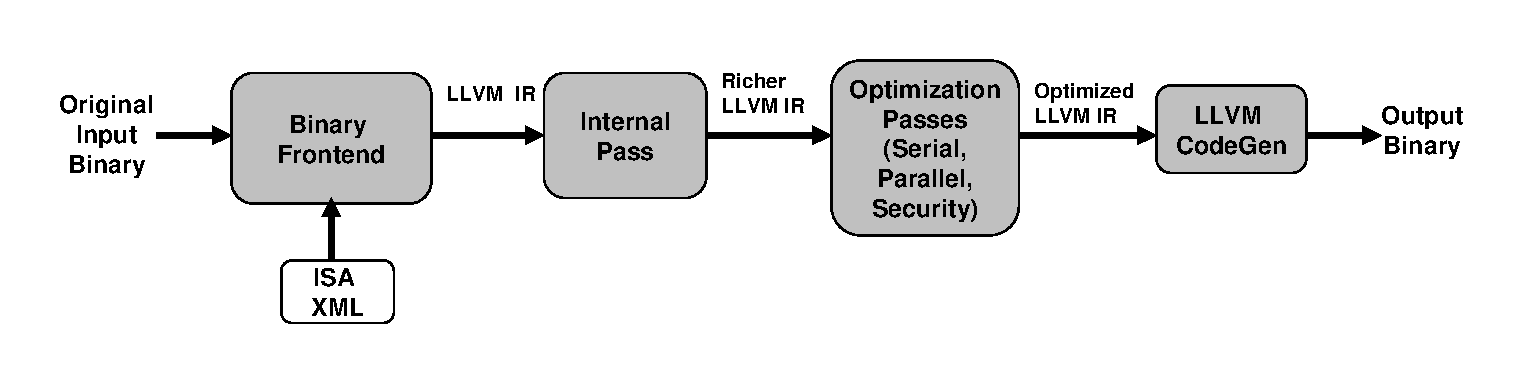
\includegraphics[scale=0.65]{sw_overview.eps}
\end{center}
\renewcommand{\baselinestretch}{1}
\small\normalsize
\begin{quote}
\caption{SecondWrite system}
\label{swoverview}
\end{quote}
\end{figure}
\renewcommand{\baselinestretch}{2}
\small\normalsize

The frontend module consists of a disassembler and a custom binary reader which processes the
individual instructions and generates an initial LLVM IR. This initial representation is void of the
desired IR features like function prototypes, abstract stack and virtual registers. The internal
pass module analyzes this initial IR to obtain an improved IR which has all the information and
features mentioned previously. Various optimization passes can be written on the above IR to obtain
an optimized IR. Finally, the optimized IR is passed to the existing LLVM code generator to obtain
the rewritten binary.

Various inherent characteristics of executables such as the unavailability of function prototypes,
the use of a phyiscal stack and the use of the set of phyiscal registers make it difficult to obtain
a high-level IR from an input executable. A number of techniques have been developed within our
group to extract this high-level information from executables whenever possible. We will not discuss
those techniques in this thesis as the techniques are explained in detail elsewhere \cite{}.

\section{Stack Canary Insertion}

The first component of our scheme is the simplest. LLVM provides the ability to insert stack
canaries during code generation. Utilizing this capability from LLVM allows us to easily provide the
same level of protection to an un-protected binary as StackGuard would provide when given an
application's source code.

Essentially, a random canary value is generated and placed on the stack during a function's prolog.
In the function epilog, the value stored on the stack is compared with the random canary value for
this process. If there is any difference, execution is halted as the canary value has been
corrupted.

While this component of our scheme is simple, it demonstrates a key advantage of SecondWrite. By
translating the input binary to LLVM's high-level intermediate representation, we were able to take
advantage of features LLVM already provides. Thus, to achieve the same level of protection as
StackGuard, we had to do very little once the binary was translated to LLVM's IR.

\section{Base Pointer Elimination}

The next component of our scheme is again due to existing LLVM optimizations. LLVM is an optimizing
compiler and the binaries produced by LLVM are highly optimized. One common optimization applied by
modern compilers on the x86 platform is to free up the EBP register for register allocation by
removing the base (or frame) pointer.

Eliminating the base pointer also removes the ability for an attacker to craft an attack by
modifying the old base pointer stored in a stack frame. In a binary which has not been compiled at a
high optimization level, base pointers may still be used. In this case, the value of the base
pointer will be pushed on the stack upon function entry in order for the value to be restored on
function return. If an attacker is able to modify the value of the base pointer, he/she could have a
fake stack frame they created be used thereby allowing the attacker to alter the flow of control of
the program.

When the base pointer is eliminated by LLVM, any attack of this form is immediately prevented. There
will be no base pointer for an attacker to modify. While corruption of the stack may still occur if
an attacker overflows a buffer in order to attempt to overwrite the base pointer, no attack will be
successful.

Again, the elimination of the base pointer highlights the advantages of SecondWrite. By utilizing an
existing compiler framework, we are able to produce highly optimized binaries which eliminate the
ability for an attacker to perform an attack on a base pointer.

\section{Return Address Protection}

Given that stack canaries as inserted by LLVM do not provide the same level of protection as the
ProPolice mechanism that comes with GCC, we decided to implement a more complete solution for
protecting against corruption of the return address.

The basic idea of our return address protection scheme is as follows:

\begin{enumerate}

 \item During the function prolog, store the return address of the current function in a global
 variable

 \item In function epilog, compare the current return address on the stack with the value saved in a
 global variable

 \item If there is any difference between these values, execution is halted

\end{enumerate}

This simple scheme will detect if the return address has been modified either directly or
indirectly. One complication with this scheme is the fact that a global variable is used for storing
the return address. If a separate global variable was created for each function, memory overhead
would become quite high. One solution is to use an array of global variables of a bounded size for
saving return values. However, if function nesting is deep as in recursive functions, issues can
still occur.

We applied an optimization for relieving this problem. We observed that this protection mechanism is
only necessary if a function contains a write to a buffer. Thus, we analyze a function to look for
any write to a buffer. If a function does not contain any write to a buffer then there is no need
for the return address protection mechanism to be inserted. During our experimental evaluation of
our scheme, we have not yet come across a recursive function, which could cause issues for our
scheme, that required return address protection to be inserted.

\section{Function Pointer Protection}

\section{longjmp/setjmp Protection}
